\documentclass[12pt,a4paper]{article}
\usepackage{ucs}
\usepackage{caption}
\usepackage[latin1,utf8x]{inputenc}
\usepackage{amsmath}
\usepackage{caption}
\captionsetup{font=small,labelfont=bf}
\usepackage[danish]{babel}
\usepackage[rmargin=3cm,tmargin=3.3cm]{geometry}
\usepackage{listings}
\usepackage{color}
\setlength{\parindent}{0pt}
\setlength{\parskip}{1ex plus 0.5ex minus 0.2ex}
\usepackage{graphicx}
\usepackage{fixltx2e}


%insert links
\usepackage{hyperref}
\usepackage{fancyhdr,lastpage}	
\pagestyle{fancy}


\definecolor{mygreen}{rgb}{0,0.6,0}
\definecolor{myblue}{rgb}{0,0,1}
\definecolor{myyellow}{rgb}{0.7,0.7,0}
\definecolor{myblack}{rgb}{0,0,0}

\lstset{
	breaklines=true,
	numbers=left, 
	commentstyle=\color{mygreen},
	stringstyle=\color{myyellow},
}

%header
\lhead{ 
	Embedded Systems \\
	02131 \\ 
}
\chead{ 
}
\rhead{ 2 October, 2012 \\ \bigskip  }

%Footer
\lfoot{
	\rule{\textwidth}{0.1mm}\\
}

\cfoot{}
\rfoot{\ \\ \scriptsize{Side \thepage\ af \pageref{LastPage}}}

\begin{document}

%Forside
\begin{titlepage}
	\begin{center}
		\vspace*{13\baselineskip}
		\huge
		\bfseries
		Embedded Systems\\ 
		\ \\
		02131 \\[5\baselineskip]

		\normalfont
		\Large
		R-peak detection!\\	
		2013

		\small
		\vfill
	\end{center}	
	\begin{flushleft}
		Jakob Welner, s124305\\
	 	Jacob Gjerstruo, s113440\\
	\end{flushleft}
\end{titlepage}

\ \\
\section*{Abstract}


\thispagestyle{empty} 
\newpage

%Table of Contents
\tableofcontents
\thispagestyle{empty} 
\newpage

%Reset pagecount
\setcounter{page}{1}

%Alm. sider
\ \\
\section{Introduction}
	After successfully proving in assignment 1 that the QRS algorithm could be implemented, Medembed now wants a proof of concept that this QRS algorithm can be implemented by using a small embedded processor. To do this, one of the filters will be implemented through the use of the Hardware Description Language (HDL) Gezel.\\
	This report will discuss how the filter will be implemented through Gezel, as well as the following topics: Modules of the processor, Instruction set for the processor, Controller for the processor, Integration of the processor into a combined system, and finally, the critical parts of the processor, i.e. speed (clock cycles per second), power consumption (watt) and size (memory requirements).\\
	
	 the to implement a small embedded processor. This processor needs to be able to execute the QRS algorithm on a proof-of-concept basis, done by implementing just one of the filters to demonstrate the performance of the processor.	
\subsection{Requirements}
Below follows a list of functional and non-functional requirements:\\

\textbf{ Functional requirements for the application:}
\begin{itemize}
	\item Each module of the processor must first be built, run and tested by their own
	\item An instruction set must be designed
	\item A controller for the instruction set must be designed
	\item The controller must be integrated into a larger system
	\item The performance of the system must be analysed in terms of speed and memory requirements

\end{itemize}
\textbf{Non-functional requirements for the application:}
\begin {itemize}
	\item The processor must be implemented with the use of Gezel
\end{itemize}

\section{Theory}
 	In order to initiate the structure- and design-process of the program, a number of questions needed to be answered first:\\
 	
 	\begin{enumerate}
	\item Which processor modules is needed and how should these be made?
	\item What instructions must the instruction set contain?
	\item How can the controller be implemented in a way such that it can understand and carry out the instruction set?
	\item How can the controller be integrate into the system?
	\item What are the critical parts of the system and how can these be analysed?
\end{enumerate}

\subsection{Problem 1: Processor modules}
	To create the processor modules, 
\subsection{Problem 2: Instruction set}
	
\subsection{Problem 3: Implementation of the controller}

\subsection{Problem 4: System Integration}

\subsection{Problem 5: Critical parts}

\section{Design}

\section{Implementation}

\subsection{Processor modules}

\subsection{Instruction set}
	
\subsection{Implementation of the controller}
	
\subsection{System Integration}
	
\subsection{Critical parts}

\section{Results}
	
%	\begin{figure}[h!]
%		\centering
%			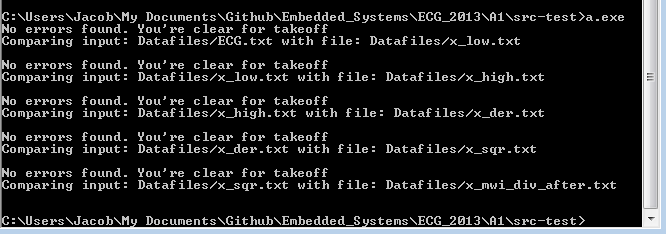
\includegraphics[width=1\textwidth]{Screenshots/tests_filter_result.png}
%		\caption{A screenshot of the output of the tests of the filters.}
%		\label{test_filter_result}
%	\end{figure}

\section{Discussion}
	
\subsection{Improvements}

\section{Conclusion}
\newpage
\begin{thebibliography}{9}

\bibitem{lamport94}
  Michael Reibel Boesen, Jan Madsen, Linas Kaminskas, Paul Pop, Karsten Juul Frederiksen\\
  \emph{Assignment 2: The ECG processor}\\
  2013.\\

\bibitem{Gezel}
  \emph{Lecture7: Finite state machine with Datapath}\\
  Fall, 2007.\\

\bibitem{GezelBasicSyntax}
  \emph{GEZEL Basic Syntax}\\
\end{thebibliography}
	
\newpage	
	\begin{Large}
		\textbf{Appendix}
	\end{Large}
	\appendix

\section{Who wrote what}
Jacob Gjerstrup, s113440 wrote: \\
Jakob Welner, s124305 wrote: \\

\section{Output of the RPeakDetection}
	
\section{Sourcecode - introductionary exercises}
	
\section{Sourcecode - the real program}

\subsection{Buffer}
	%\lstinputlisting[language=C]{Code/buffer.c}	
\subsection{Filters}
\subsection{RPeakDetection}
\subsection{Sensor}
\subsection{Header files}
\subsubsection{sensor.h}
\subsubsection{buffer.h}
\subsection{Tests}
\end{document}